\section{\texorpdfstring{STM8S105C6}{STM8S105C6}}

% =====================================================================================================================
	\begin{frame}
    \frametitle{STM8S105C6 - datasheet}
		
		\begin{itemize}
			\item 16 MHz,
			\item 3 stavová Pipeline,
			\item Harvardská architektura:
			
			\begin{itemize}
				\item Programová paměť FLASH: 32 kB
				\item Pamět pro data nevolatilní EEPROM: 1 kB
				\item Pamět pro data volatilní RAM: 2 kB
			\end{itemize}
			\item Napájení 2.95 V až 5.5 V
			\item Periférie: ADC (10 bit), I2C, SPI, UART, ...
		\end{itemize}
		
		\vspace{3mm}
		Odkaz na datasheet je také na Moodlu: \textcolor{blue}{\url{https://www.st.com/resource/en/datasheet/stm8s105c6.pdf}}

	\end{frame}
	
% =====================================================================================================================
	\begin{frame}
    \frametitle{STM8S105C6 - periferie}
		
		\begin{center}
			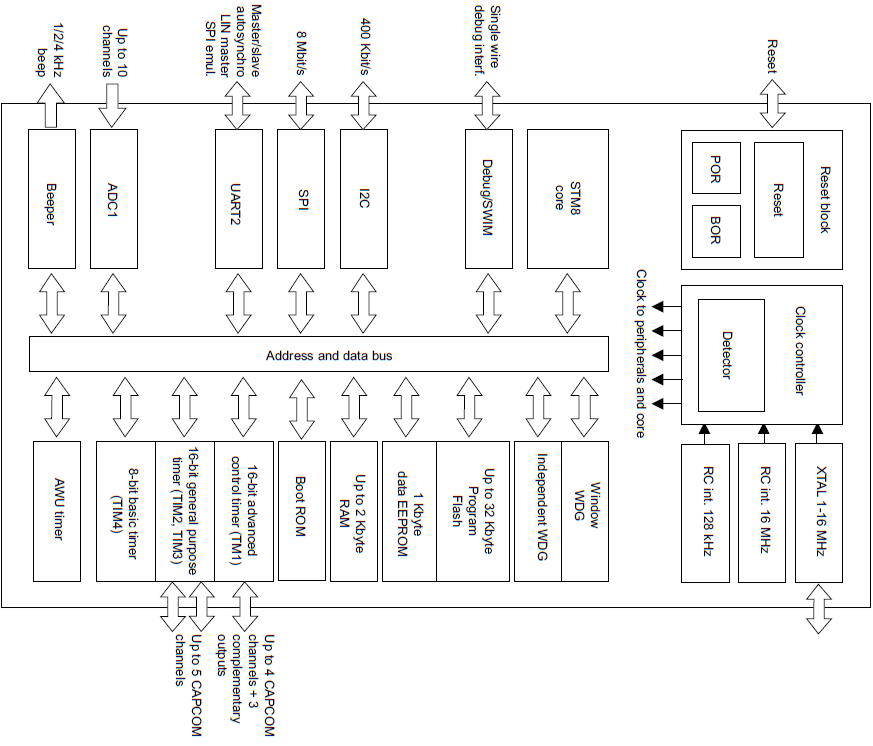
\includegraphics[width=0.7\textwidth]{fig/peripherals.png}
		\end{center}

	\end{frame}
	
% =====================================================================================================================
	\begin{frame}
    \frametitle{STM8S105C6 - paměť}
		
		\begin{center}
			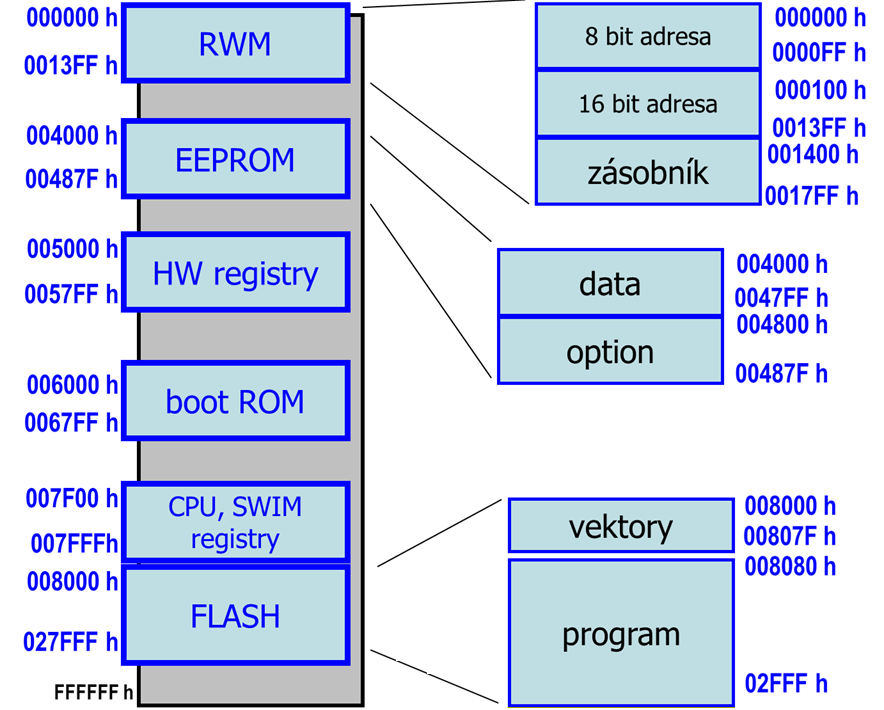
\includegraphics[width=0.65\textwidth]{fig/memory_map.png}
		\end{center}

	\end{frame}
	
% =====================================================================================================================
	\begin{frame}
    \frametitle{STM8S105C6 - programátorský model}
		
		\begin{center}
			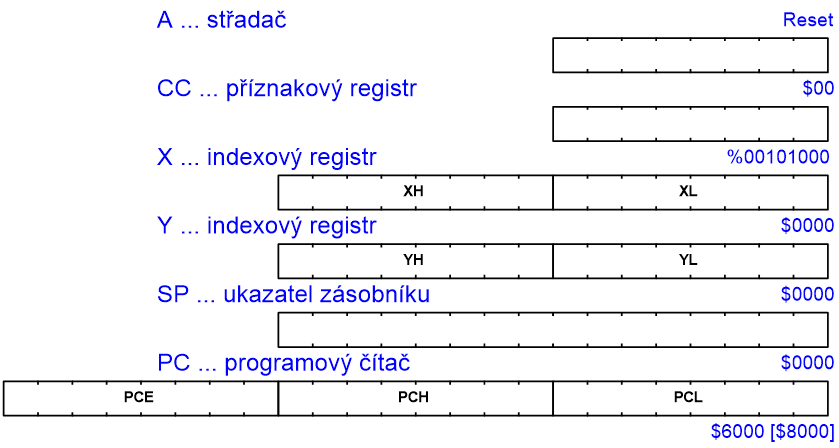
\includegraphics[width=\textwidth]{fig/registers.png}
		\end{center}

	\end{frame}

% =====================================================================================================================
	\begin{frame}
    \frametitle{STM8S105C6 - programátorský model}
		
		\begin{itemize}
			\item \textbf{A střadač} ... také akumulátor, pracovní registr používaný ALU při aritmetických a logických operacích. \vspace{3mm}
			\item \textbf{CC příznakový registr} ... jednotlivé bity odpovídají určitým příznakům specifikující výsledek poslední provedené  operace. \vspace{3mm}
			
			\begin{center}
				\begin{tabular}{|c|c|l|}
					\hline
					7 & V & aritmetické přetečení \\
					\hline
					6 &  &  \\
					\hline
					5 & I1 & maska přerušení, úroveň 1 \\
					\hline
					4 & H & poloviční přetečení, přenos ze spodní nible \\
					\hline
					3 & I0 & maska přerušení, úroveň 0 \\
					\hline
					2 & N & znaménko, záporný výsledek \\
					\hline
					1 & Z & nulový výsledek \\
					\hline
					0 & C & přenos, pro byte \\
					\hline
				\end{tabular}
			\end{center}
		\end{itemize}

	\end{frame}
	
% =====================================================================================================================
	\begin{frame}
    \frametitle{STM8S105C6 - programátorský model}
		
		\begin{itemize}
			\item \textbf{X, Y indexové registry} ... lze použít jako obecné registry, používají se pro indexové adresování (tabulky) \vspace{3mm}
			\item \textbf{SP ukazatel zásobníku} ... ukazuje na vrchol zásobníku (STACK), což je paměť typu LIFO určená převážně pro uchovávání návratových adres funkcí a přerušení. \vspace{3mm}
			
			\item \textbf{PC programový čítač} ... ukazuje na právě vykonávanou (dekódovanou) instrukci. \vspace{3mm}
		\end{itemize}

	\end{frame}
	
% =====================================================================================================================
	\begin{frame}
    \frametitle{STM8S105C6 - přípravek na cvičení}
		
		\begin{center}
			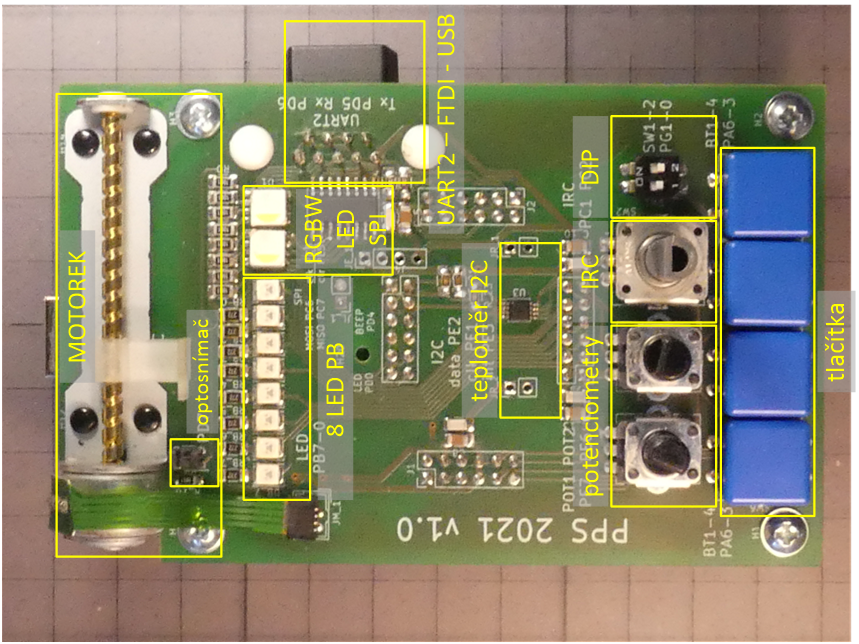
\includegraphics[width=0.80\textwidth]{fig/mcu_kit.png}
		\end{center}

	\end{frame}
	
% =====================================================================================================================
	\begin{frame}
    \frametitle{STM8S105C6 - výběr ladicích prostředků}
		
		\begin{center}
			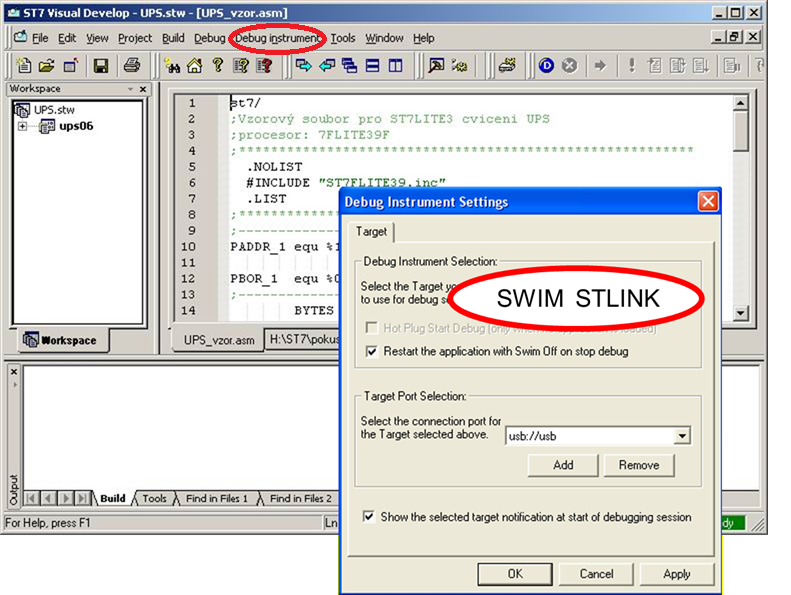
\includegraphics[width=0.90\textwidth]{fig/mcu_kit_debug.png}
		\end{center}

	\end{frame}